
% --------------------------------------------------------------- CONFIGURATIONS

\documentclass[a4paper,12pt,final,oneside]{book}

\usepackage{rapport}


% -------------------------------------------------------------- META: CONSTANTS

\newcommand{\reporttitle}{Grammaire et langage}
\newcommand{\enseignants}{Nabila~\textsc{Benharkat}\\Eric~\textsc{Guérin}}
\newcommand{\reportauthor}{Guillaume~\textsc{Abadie}\\Thierry~\textsc{Cantenot}\\Juliette~\textsc{Courlet}\\Rémi~\textsc{Domingues}\\Adrien~\textsc{Duffy-Coissard}\\Ahmed~\textsc{Kachkach}}
\newcommand{\reportsubject}{Livrable de projet}
\newcommand{\stagetopic}{Analyse de fichiers XML}
\newcommand{\dateperiod}{du 14 Mars au 3 Mars 2014}
\newcommand{\HRule}{\rule{\linewidth}{0.5mm}}
\setlength{\parskip}{1ex} % Espace entre les paragraphes

\hypersetup{
	pdftitle={\reporttitle},%
		pdfauthor={\reportauthor},%
		pdfsubject={\reportsubject},%
		pdfkeywords={INSA Lyon} {Grammaire et langage}
}

\title{\reporttitle}
\author{\reportauthor}
%\setcounter{tocdepth}{4}


% ------------------------------------------------------------------------- FILE

\begin{document}


    % ------------------------------------------------------------------- HEADER

	\renewcommand{\chaptername}{} %\renewcommand{\thechapter}{}
	\renewcommand{\contentsname}{Sommaire}

	\pagestyle{empty}
	\pagenumbering{Roman}


    % ------------------------------------------------------------ HEADER: TITLE

	% Inspiré de http://en.wikibooks.org/wiki/LaTeX/Title_Creation
\begin{center}
	\begin{minipage}[t]{0.48\textwidth}
	  \begin{flushleft}
	    
\includegraphics [width=40mm]{images/logo_INSA.png} \\[0.5cm]
			INSA Lyon\\
			20, avenue Albert Einstein\\
			69621 Villeurbanne Cedex
	  \end{flushleft}
	\end{minipage}
	\begin{minipage}[t]{0.48\textwidth}
	  \begin{flushright}
	    %\includegraphics [width=60mm]{images/logo_Passau.jpg} \\[0.5cm]
	    %Universität Passau\\
		%Innstraße, 3\\
		%	D-94032 Passau
	  \end{flushright}
	\end{minipage} \\[2cm]

	\textsc{\Large \reportsubject}\\[0.3cm]
	\HRule \\[0.4cm]
	{\Huge \bfseries \reporttitle}\\[0.3cm]
	{\LARGE \bfseries «~\stagetopic~»}\\[0.3cm]
	{\Large \dateperiod}\\[0.4cm]
	\HRule \\[1cm]

	
\includegraphics [scale=0.35]{images/application-xml.png} \\[0.7cm]
	\begin{minipage}[t]{0.4\textwidth}
	  \begin{flushleft} \large
	    \emph{Hexanôme~:}\\
	    \small \reportauthor
	  \end{flushleft}
	\end{minipage}
	\begin{minipage}[t]{0.5\textwidth}
	  \begin{flushright} \large
	    \emph{Enseignants~:} \\
	    \enseignants
	  \end{flushright}
	\end{minipage}

	\vfill
	\footnotesize{Année scolaire 2013-2014}
\end{center}



    % --------------------------------------------------- HEADER: CONFIGURATIONS

	\sloppy          % Justification moins stricte : des mots ne dépasseront pas des paragraphes

    \frontmatter
		\pagestyle{empty}
		\tableofcontents
		\addtocontents{toc}{\protect\thispagestyle{empty}}

	\mainmatter
	\pagestyle{headings}

	\renewcommand{\chaptermark}[1]{\markboth{\MakeUppercase{\chaptername\ \thechapter.\ #1}}{}}
	\renewcommand{\sectionmark}[1]{\markright{\thesection{} #1}}


    % ------------------------------------------------------------------ CONTENT

	\chapter{Introduction}

L'objectif de ce projet est de réaliser un processeur xml en C++, en utilisant en plus les outils flex et bison. Ceux-ci nous permettront d'analyser syntaxiquement et sémantiquement le langage xml, afin de créer une grammaire simplifiée. Notre programme a 3 fonctionnalités principales : parser un fichier xml et l'afficher, valider un document xml par rapport à un document xsd, et enfin transformer un document xml avec une feuille de style xsl. En raison du temps qui est imparti pour ce projet, ces fonctionnalités ne couvriront pas toutes les possibilités offertes par le langage xml, afin de réduire le temps de développement de ce programme. \\
Nous l'utiliserons en ligne de commande de la façon suivante :
\begin{description}
    \item[Parsage/affichage du fichier doc.xml~:] ~\\
        \lstinline$xmltool -p doc.xml$
    \item[Validation du fichier doc.xml par rapport au fichier doc.xsd!:] ~\\
        \lstinline$xmltool -v doc.xml doc.xsd$
    \item[Transformation du fichier doc.xml avec la feuille de style doc.xsl~:]~\\
        \lstinline$xmltool -t doc.xml doc.xsl$ \\
\end{description}

Voici l'architecture global de notre programme :

    \begin{figure}[h!]
        \centering
        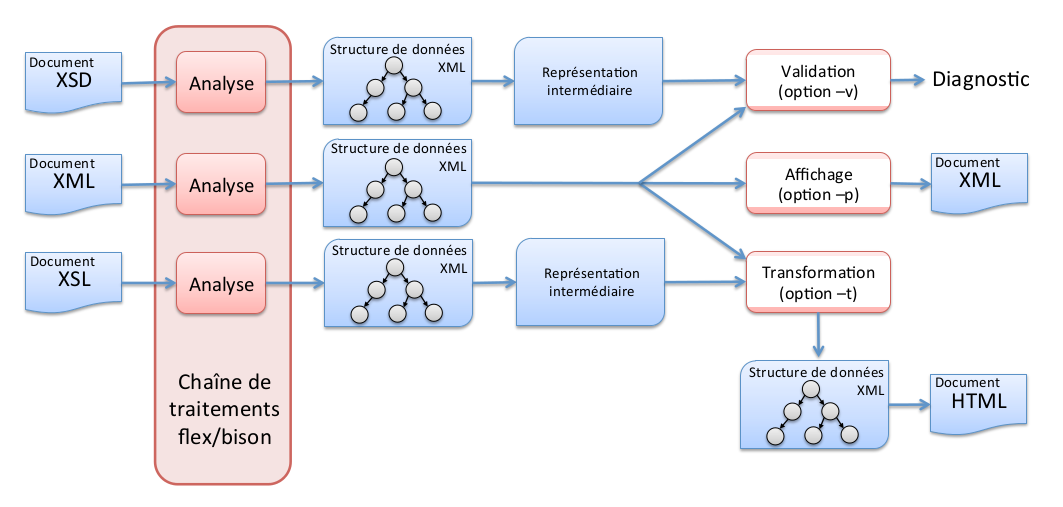
\includegraphics[width=0.8\linewidth]{images/archi.png}
        \caption{Architecture globale}
        \label{classDiagram}
    \end{figure}

La conception sera détaillée plus précisément dans la suite du document.

	\chapter{Namespace XML}

Cette partie décrit la représentation C++ d'un XML ainsi que les traitements associés.

Les hypothèse suivantes sont également formulées :
\begin{itemize}
    \item Les documents XML à parser ne contiendront pas de DTD interne
    \item Les Processing Instruction (PI) ne contiendront que des attributs
    \item Aucune référence ne sera présente dans les documents XML\\
\end{itemize}


\section{Diagramme de classes}
    Les classes ici décrites seront rattachées au \textit{\lstinline$namespace Xml$} défini en C++.

    \begin{landscape}
    \begin{figure}[h!]
        \centering
        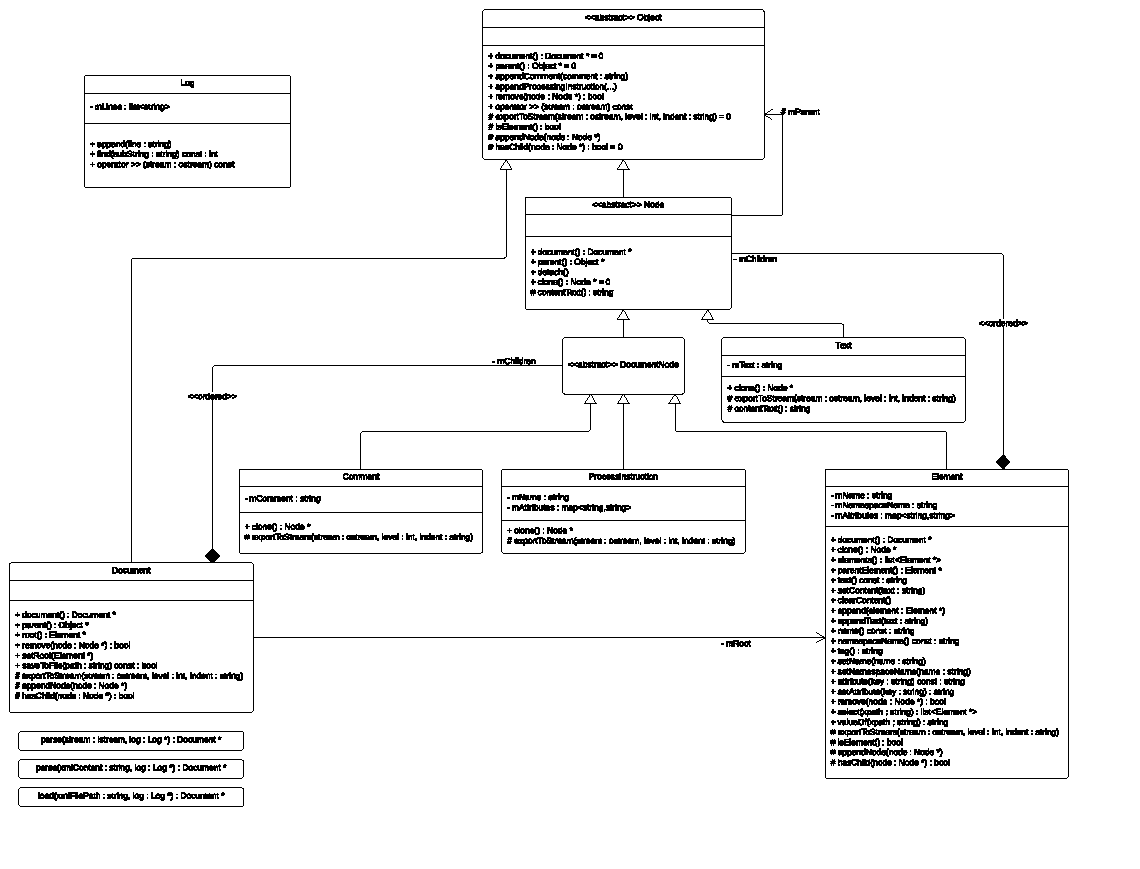
\includegraphics[width=0.9\linewidth]{images/xml-uml.pdf}
        \caption{Diagramme de classes de l'arborescence XML}
        \label{classDiagram}
    \end{figure}
    \end{landscape}


\section{Classes}
    \subsection{Log}
        La class \lstinline$Log$ a pour unique mission de stocker l'ensemble de l'output du parseur \textit{XML} telle que~:

        \begin{itemize}
            \item Erreurs lexicales~;
            \item Erreurs syntaxique~;
            \item Erreurs semantiques.
        \end{itemize}

    \subsection{Object}
        Pour optimiser et éviter au maximum la redondance de données dans notre arbre d'héritage de l'implementation \textit{XML}, nous nous sommes inspirés de la très célèbre librarie \textit{Qt} avec son \lstinline$QObject$. Ainsi nous avons notre \lstinline$Xml::Object$ offrant les avantages que vous trouverez dans les sous-sections suivantes.

    \subsection{Node}
    Ainsi, nous partons du principe qu'un document XML n'est en réalité qu'un arbre ayant des noeuds (\lstinline$Node$) étant des objects XML, mais de natures differents (commentaires, texte, élément \ldots). Certains de ces noeuds seront des feuilles de l'arbre (le noeud de commentaire par exemple).

        Ici se trouve déjà un avantage du \lstinline$Xml::Object$ car chaque \lstinline$Node$ connait son \lstinline$Object$ parent à l'aide de \lstinline$mParent$ pouvant être un \lstinline$Element$ ou un \lstinline$Document$. Ainsi, on peut à partir d'un noeud, retrouver le \lstinline$Document$ dans lequel il se trouve simplement en remontant l'arbre.

    \subsection{DocumentNode}
        Le \lstinline$DocumentNode$ est une spécialisation de \lstinline$Node$, mais ayant seulement une particularité' sémantique~: seul ses classes fillent peuvent avoir pour parent, un \lstinline$Element$ par hertiage de \lstinline$Node$, mais aussi un \lstinline$Document$ au contraire de la classe \lstinline$Text$ ne pouvant avoir pour parent qu'un \lstinline$Element$.

    \subsection{Document}
        Un \lstinline$Document$ est un \lstinline$Node$ composé de \lstinline$DocumentNode$. Parmis ces \lstinline$DocumentNode$, un seul et unique \lstinline$Element$ racine compose cette liste. Mais afin de pouvoir retrouver cette racine du document en complexité $O(1)$, \lstinline$DocumentNode$ dispose aussi d'un attributs \lstinline$mRoot$ dedié à cette tache.

        Cette même liste de \lstinline$DocumentNode$ est ordonnée afin de garentir l'ordre des noeuds au chargement et à l'exportation du document \textit{XML}. L'\lstinline$Element$ racine fait partie de cette liste afin d'éviter d'avoir à gerer deux listes de noeuds (ceux avant et ceux après).

    \subsection{Comment}
        \lstinline$Comment$ est un \lstinline$DocumentNode$ car il peut être n'importe où dans le document \textit{XML}~: dans un \lstinline$Element$ ou bien en dehors de l'élément racine du document.

    \subsection{ProcessingInstruction}
        Une \lstinline$ProcessingInstruction$ est aussi un \lstinline$DocumentNode$ d'après les spécifications officielles de \textit{XML}. Mais en accord avec l'hypothèse énoncée précédemment, une \lstinline$ProcessingInstruction$ ne contient qu'un nom et une map d'attributs.

    \subsection{Text}
        Un noeud de texte est naturellement décrit par une chaîne de caractères \lstinline$mText$. Celui-ci ne dérive pas de la classe \lstinline$DocumentNode$ puisque, si son contenu s'apparente à celui d'un noeud Comment, il ne peut en revanche être contenu par une instance de \lstinline$Element$. Il est donc nécessaire d'ajouter le niveau de spécialisation \lstinline$DocumentNode$ afin d'éviter une relation ne respectant pas les spécifications standards \textit{XML}.

    \subsection{Element}
        Un \lstinline$Element$ \textit{XML} est un \lstinline$DocumentNode$. Il possède une liste d'\lstinline$Element$ enfants \lstinline$mChildren$. Cette classe peut aussi représenter la racine d'un \lstinline$Document$.

        Celui ci est defini avec un nom de balise (\lstinline$mName$) mais aussi d'un espace de nom (\lstinline$mNamespaceName$). La concatenation de ces deux derniers forment le tag (namespace + ":" + nom) de l'\lstinline$Element$. Le nom du membre \lstinline$mNamespaceName$ au lieu de \lstinline$mNamespace$ a été effectué pour éviter la collision avec le mot clef du language C++ \lstinline$namespace$ avec son getter théorique \lstinline$Xml::Element::namespace()$ remplacer par \lstinline$Xml::Element::namespaceName()$.

        Un \lstinline$Element$ possède un ensemble non-ordonné d'attributs étant simplement une map ayant une association $clef \leftarrow valeur$. Par soucis de déterminisme, nous les exportons par ordre alphabétique des clefs.

        Enfin un \lstinline$Element$ possède une liste ordonnée de noeuds (\lstinline$Node$). Mais cette liste est inaccessible à l'utilisateur. En effet, nous ne voulons pas que l'utilisateur du namespace ait besoin de tester les différents types de noeuds.
        La méthode \lstinline$Xml::Element::elements()$ permet de récupérer l'ensemble des \lstinline$Element$ fils.

    /* FIXME */


        Mais il ne pourra pas recuperer les \lstinline$Comment$ car ne sont pas senser être parser. De même l'utilisateur ne pourra acceder aux \lstinline$ProcessingInstruction$ car sont seulement dedier au parser \textit{XML}.

    /* END FIXME */

        L'utilisateur pourra accéder au contenu texte d'un \lstinline$Element$ à l'aide de \lstinline$Xml::Element::text()$ qui concatènera l'ensemble des noeuds enfants de type \lstinline$Text$.


\section{Encapsulation du namespace Xml}
    Au final l'utilisateur aura simplement accès aux classes suivantes~:

    \begin{itemize}
        \item \lstinline$Log$~;
        \item \lstinline$Object$~;
        \item \lstinline$Document$~;
        \item \lstinline$Element$.
    \end{itemize}

    Les autres classes sont implémentées avec des constructeurs \lstinline$private$ (avec des amitiés nécessaires entre elles bien entendu). Ainsi l'utilisateur peut réutiliser notre implémentation tout aussi facilement que la librarie \lstinline$DOM$ ayant pour avantage de ne pas avoir à gérer la présence de commentaires ou de processing instructions dans son code car ne travaillant dans l'arbre \textit{XML} qu'avec \lstinline$Document$ et \lstinline$Element$.
    \\
    \begin{lstlisting}[frame=single]
Xml::Document doc;

doc.setRoot(new Xml::Element("root"));
doc.root()->append(new Xml::Element("hi"));
doc.root()->appendComment("Hello world!");
doc.root()->append(new Xml::Element("bar", "foo"));

assert(doc.elements("hi").size() == 1);

doc.elements()[1]->setAttribute("attr", "myValue");

delete doc.elements("hi")[0];

std::cout << doc << std::endl;
/** stdout:
 * <root>
 *   <!--Hello world!-->
 *   <foo:bar attr="myValue"/>
 * </root>
 */
    \end{lstlisting}


\section{Algorithmes}

    \subsection{Xml::Element::select}

    \textbf{\lstinline$std::list<Xml::Element const *> Xml::Element::select(std::string const \& xPathQuery) const$}

    Dans la suite de cette section, nous nous référerons à l'élément sur lequel nous appelons \lstinline$Xml::Element::select$ par "E".

    \subsubsection{Description}
    Cette méthode permet de récupérer la liste des éléments matchant une requête XPath.

    Les requêtes XPath supportés sont les suivantes :
    \begin{itemize}
        \item \textit{""} : Retourne une liste vide.
        \item \textit{"/"} : Retourne une liste contenant la racine du document si E fait partie d'un document, une liste vide sinon.
        \item \textit{"."} : Retourne une liste contenant E.
        \item \textit{".."} : Retourne une liste contenant le parent de E si le parent est un élément, une liste vide sinon.
        \item \textit{"bookstore"} : Retourne liste des éléments enfants de E qui ont pour tag \textit{bookstore}.
        \item \textit{"bookstore/book"} : Retourne la liste des éléments qui sont des \textit{book} enfants de \textit{bookstore} enfants de E.
        \item \textit{"/bookstore/book"} : Retourne la liste des éléments qui sont des \textit{book} enfants de \textit{bookstore} qui sont enfants de la racine du document si E appartient à un document, une liste vide sinon.
        \\
    \end{itemize}

    Dans le cas où aucun élément ne match la requête, une liste vide est renvoyée.

    \subsubsection{Algorithme}

    Pour la suite, nous nous référerons à la requête XPath par "XP".

    Le fonctionnement de l'algorithme \lstinline$Xml::Element::select$ est le suivant :
    On regarde si XP est égale à "", "/", "." ou ".." ce qui correspond aux 4 premiers cas triviaux cités précedemment.
    Si XP se trouve parmi ces 4 cas, le traitement est immédiat et retourne ce qui a été définis au-dessus.

    Sinon, on regarde si XP possède un "/" :
    \begin{itemize}
        \item Si XP ne possède pas de "/", XP est un tag simple et on cherche, parmi les éléments de E, les éléments qui ont pour tag XP et on les renvoie dans une liste.
        \item Si XP possède moins un "/" mais ne commence pas par un "/", il s'agit d'un chemin relatif par rapport à E. Dans ce cas, on extrait la chaîne partant du début de XP jusqu'au premier "/" et on récupère tous les enfants de E qui possède ce tag. Ensuite, on appelle récursivement \lstinline$Xml::Element::select$ sur chacun des éléments avec pour requête XPath la sous-chaîne de XP commençant juste après le premier "/" jusqu'à la fin de XP. On concatène ensuite toutes les listes récupérées via les appels à \lstinline$Xml::Element::select$, puis on renvoie la nouvelle liste générée.
        \item Si XP possède au moins un "/" et commence par "/", on appelle \lstinline$Xml::Element::select$ sur la racine du document contenant E avec pour requête XP privée de son premier "/". On se retrouve alors dans le cas précédent avec E étant la racine.
        \\
    \end{itemize}

    Dans le cas où aucun élément ne match la requête, une liste vide est renvoyée.

    \subsection{Xml::Element::valueOf}

    \textbf{\lstinline$std::string Xml::Element::valueOf(std::string const \& xPathQuery) const$}

    Dans la suite de cette section, nous nous référerons à l'élément sur lequel nous appelons \lstinline$Xml::Element::valueOf$ par "E".

    \subsubsection{Description}
    Cette méthode permet de récupérer la valeur d'une requête XPath.

    Les requêtes XPath supportés sont les suivantes :
    \begin{itemize}
        \item \textit{""} : Retourne une chaîne vide.
        \item \textit{"/"} : Retourne le texte contenu récursivement de la racine.
        \item \textit{"bookstore"} : Retourne le texte contenu récursivement du premier élement enfant de E qui a pour tag \textit{bookstore}.
        \item \textit{"bookstore/book"} : Retourne le texte contenu récursivement du premier élement des \textit{book} enfants de \textit{bookstore} enfants de E.
        \item \textit{"/bookstore/book"} : Retourne le texte contenu récursivement du premier élement des \textit{book} enfants de \textit{bookstore} qui sont enfants de la racine du document.
        \item \textit{"@attr"} : Retourne la valeur de l'attribut \textit{attr} de E.
        \item \textit{"/@attr"} : Retourne la valeur de l'attribut \textit{attr} de la racine du document ou une chaîne vide.
        \item \textit{"bookstore/@attr"} : Retourne la valeur de l'attribut \textit{attr} du premier élement enfant de E qui a pour tag \textit{bookstore}.
        \item \textit{"bookstore/book/@attr"} : Retourne la valeur de l'attribut \textit{attr} du premier élement des \textit{book} enfants de \textit{bookstore} enfants de E.
        \item \textit{"/bookstore/book/@attr"} : Retourne la valeur de l'attribut \textit{attr} du premier élement des \textit{book} enfants de \textit{bookstore} qui sont enfants de la racine du document.
        \\
    \end{itemize}

    Dans le cas où un attribut ou un élément n'existe pas, une chaîne vide est renvoyée.

    \subsubsection{Algorithme}

    Pour la suite, nous nous référerons à la requête XPath par "XP".

    Le fonctionnement de l'algorithme \lstinline$Xml::Element::valueOf$ est le suivant :

    On regarde si XP est de la forme "", "/", "tag", "tag1/tag2" ou "/tag1/tag2".
    Dans ces cas là, on effectue un \lstinline$Xml::Element::select$ avec XP comme requête.
    On récupère ensuite tout le texte contenu récursivement dans le premier élément du résultat de la requête.

    Dans les autres cas, on cherche à récupérer la valeur d'un attribut. Notre approche est la suivante :
    \begin{itemize}
        \item Si XP est de la forme "@attr", on retourne la valeur de l'attribut \textit{attr} de E.
        \item Si XP est de la forme "/@attr", on retourne la valeur de l'attribut \textit{attr} de la racine du document.
        \item Dans les 3 cas restants ("tag/@attr", "tag1/tag2/@attr" et "/tag1/tag2/@attr"), on effectue un \lstinline$Xml::Element::select$ avec XP privé de "/@attr" comme requête.
        On récupère ensuite tout le texte contenu récursivement dans le premier élément du résultat de la requête.
        \\
    \end{itemize}

    Dans le cas où un attribut ou un élément n'existe pas, une chaîne vide est renvoyée.


    \subsection{Xml::Element::matches}

    \textbf{\lstinline$bool Xml::Element::matches(std::string const \& xPathQuery) const$}

	\chapter{XSD}

Dans cette partie, nous expliquerons notre conception de la partie validation d'un document XML à partir d'un document XSD.

\section{Hypothèses simplificatrices}
	Afin de simplifier l'implémentation du parseur XSD, les hypothèses suivantes ont été posées :
	\begin{itemize}
		\item{Les types simples seront de type \textit{string} ou \textit{date}}
		\item{Les types complexes seront de type \textit{sequence} ou \textit{choice} et pourront contenir des attributs}
	\end{itemize}

\section{Fonctionalités implémentées}
Les points suivants sont pris en charge par le validateur XSD :
\begin{itemize}
    \item{Choix d'éléments racine multiples}
    \item{Présence et type des attributs}
    \item{Éléments de types \textit{mixed}}
    \item{Types complexes contenant des éléments \textit{sequence} et \textit{choice} imbriqués}
    \item{Nombre d'occurences minimum et maximum par élément}
    \item{Références sur des attributs, éléments et types}
\end{itemize}

\section{Diagramme de classes}
Les classes ici décrites seront rattachées au \textit{\lstinline$namespace Xsd$} défini en C++.

\begin{landscape}
\begin{figure}[H]
	\centering
	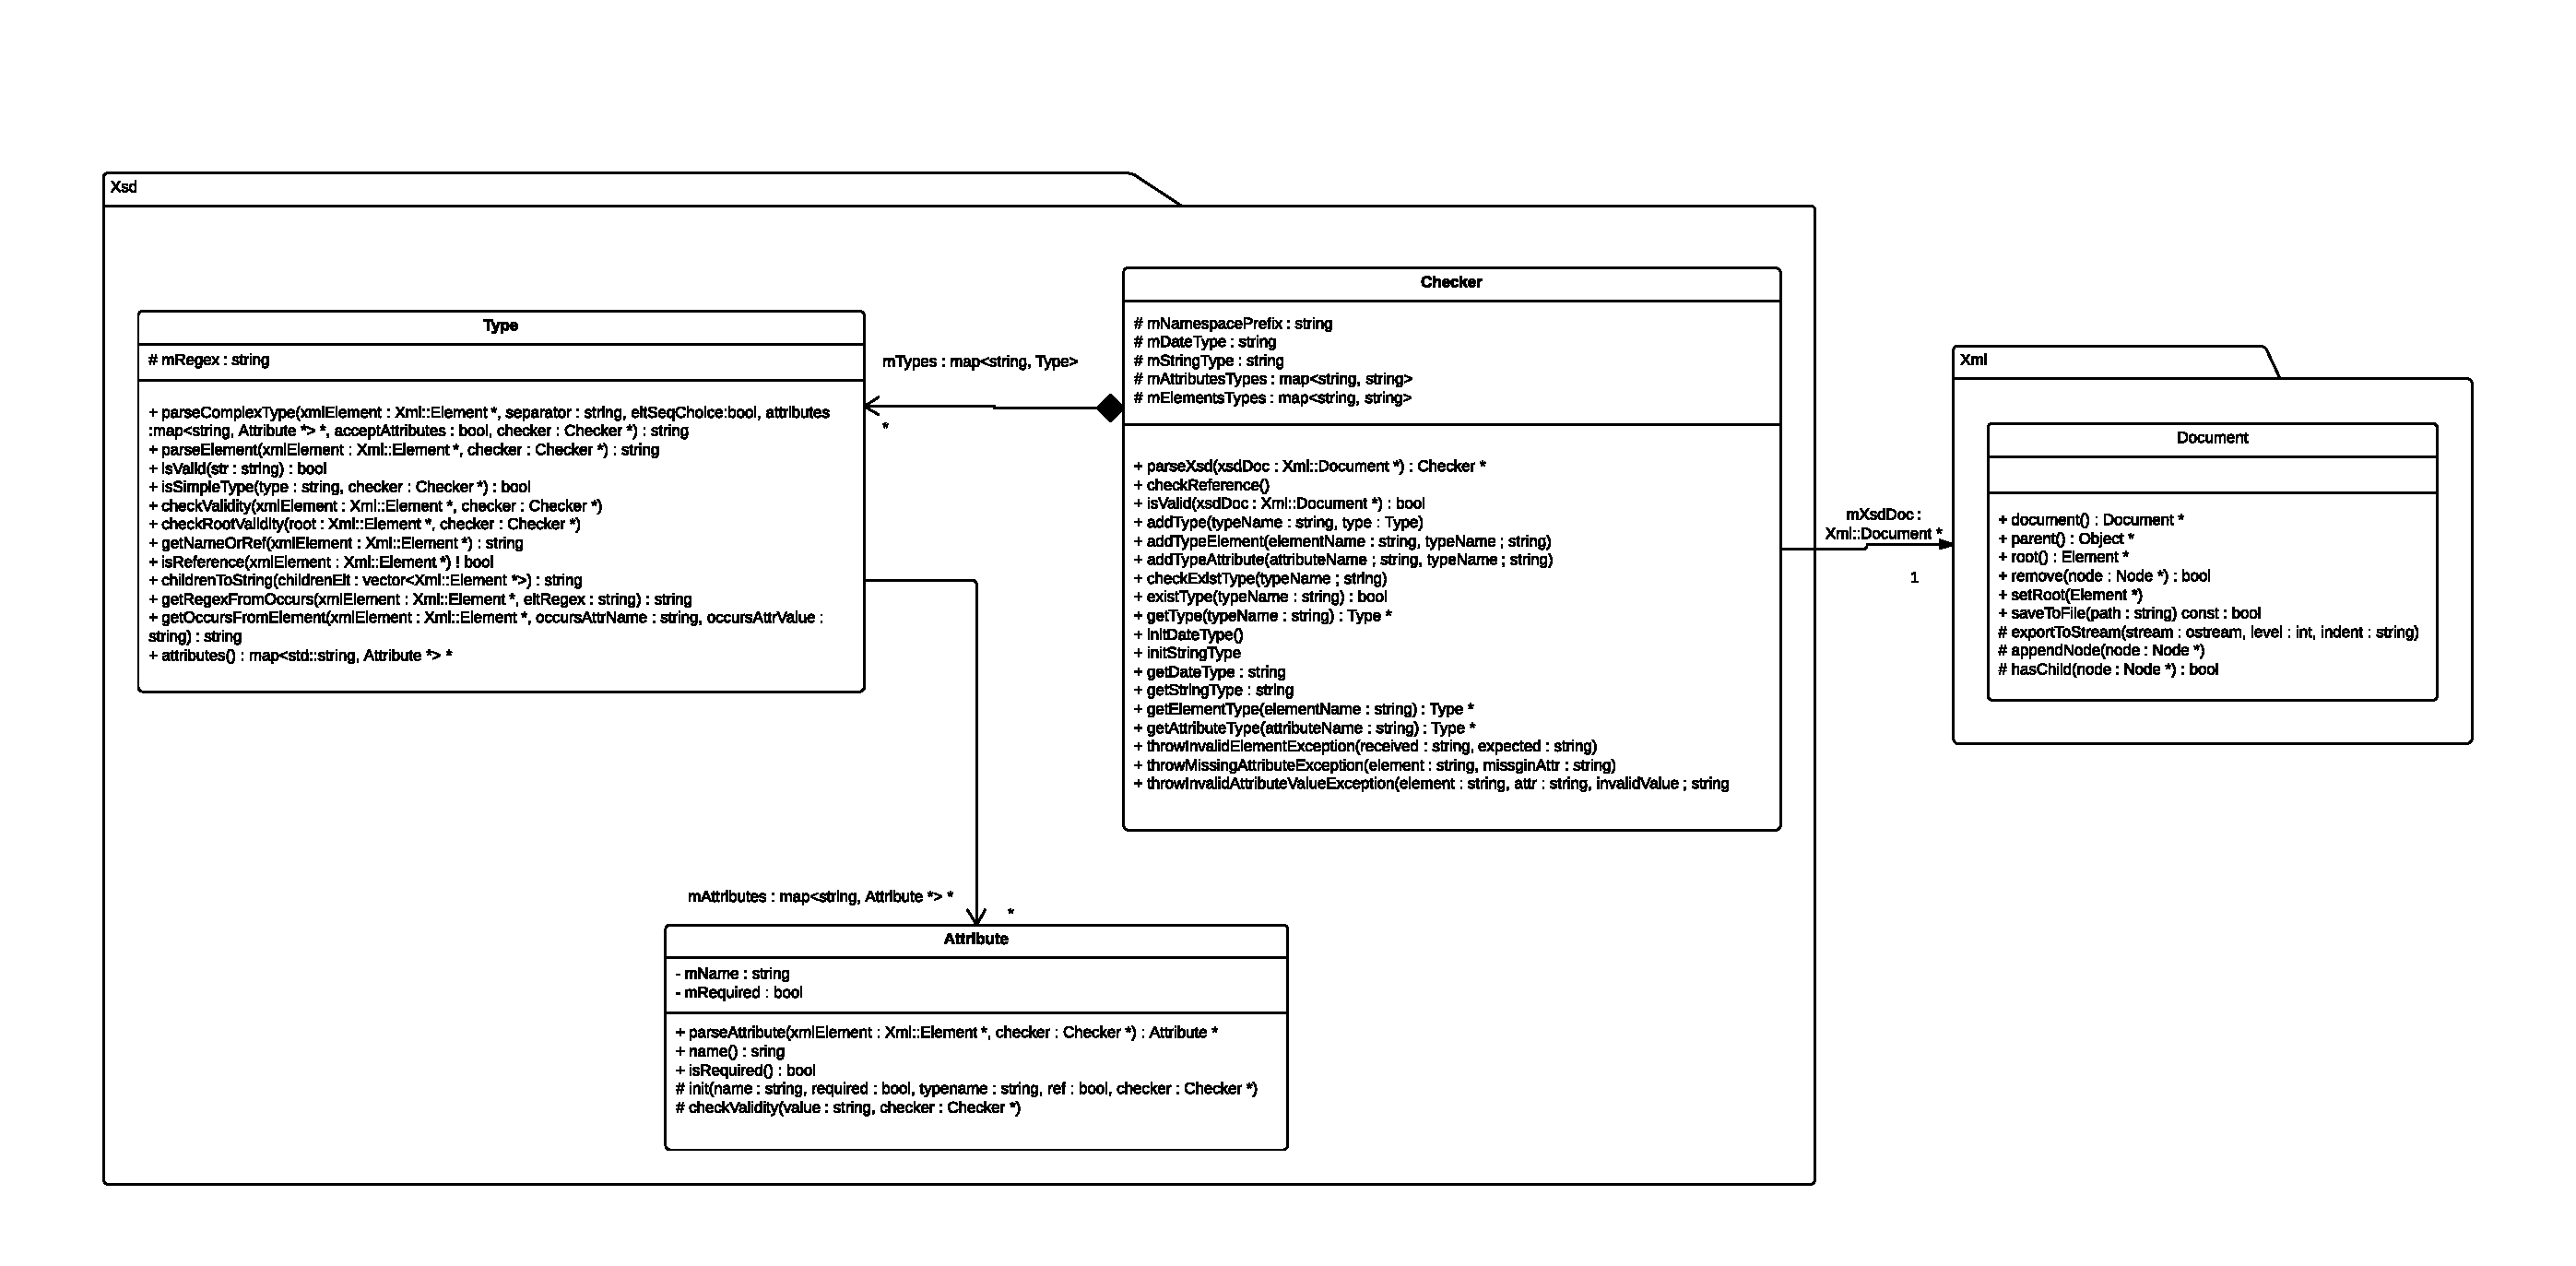
\includegraphics[width=1\linewidth]{images/xsd-uml.pdf}
	\caption{Diagramme de classe de la validation xsd}
	\label{xsdClassDiagram}
\end{figure}
\end{landscape}

\section{Entités}
	\subsection{Checker}
		Un objet Checker décrit les règles présentes dans un document XSD. Les méthodes principales sont les suivantes :
		\begin{itemize}
			\item \textbf{parseXsd} : méthode statique retournant un objet de type \textit{Checker},  construit à partir du document XSD passé en paramètre
			\item \textbf{isValid} : retourne \textit{true} si le document XML passé en paramètre est en accord avec les contraintes inscrites dans l'objet \textit{Checker} courant, \textit{false} sinon
		\end{itemize}

		La structure intermédiaire s'appuie sur 3 tables de hachages :
		\begin{itemize}
			\item \textbf{mTypes} : associe le nom (chaîne de caractères) d'un type avec son objet de type \textit{Type}
			\item \textbf{mElementsTypes} : associe le nom d'un élément avec le nom de son type
			\item \textbf{mAttributesTypes} : associe le nom d'un attribut avec le nom de son type
		\end{itemize}

	\subsection{Element}
		Un élément est une chaîne de caractères, associé\footnote{Dans la suite de cette partie, le terme \textit{associer} correspondra à l'insertion d'une paire clé/valeur dans une table de hachage} à un type dans la table de hachage \textit{mElementsTypes} d'un objet de type \textit{Checker}.

	\subsection{Type}
		On objet \textit{Type} correspond à un type complexe XSD. Il est défini par deux éléments :
		\textit{Expression régulière} : Cette chaîne de caractères détermine l'ensemble des fils directs que l'élément rattaché au type peut recevoir. Elle spécifie leur ordre et nombre d'occurences.
			\textbf{Exemple} : \textit{(<fromage>){4}|(<poisson>){1})} sera l'expression régulière du type associé à l'élément \textit{pizza}.
			Elle indique qu'une pizza peut contenir 4 fromages ou un poisson.
		\textit{Liste d'attributs} : Cette liste décrit les attributs que contiendra l'élément rattaché au type courant, l'ordre des attributs n'ayant pas d'importance.

	\subsection{Attribute}
		Un attribut est décrit par son nom et un attribut \textit{required} à \textit{true} ou \textit{false}. Il est également associé à un type dans la table de hachage \textit{mAttributesTypes}.

\section{Algorithme}

\subsection{Construction de la structure intermédiaire}
L'algorithme présent construit un objet Checker, lequel contiendra un ensemble de types et attributs.
Cet algorithme parcours en une passe l'arbre XML obtenu lors du parsing préalable du document XSD.
Il s'agît d'un algorithme récursif, le parcours de l'arbre XML pouvant être assimilé à un parseur de type SAX sur le document XSD.

	\subsubsection{Parsing du document XSD : \textit{parseXsd}}
		\lstinline$Parsing du document XSD sous forme d arbre XML$\\
		\lstinline$Parsing du type de l element racine (c.f. parseComplexType)$\\ \footnote{L élément \textit{schema} est implicitement de type complexe, ses éléments fils sont traités comme s ils étaient dans un élément \textit{choice}}
		\lstinline$Association du "ROOT_TYPE" avec le type recu$\\
		\lstinline$Association du nom d element "ROOT" avec le type recu$\\
		\lstinline$Verification des references (c.f. checkReferences)$\\

	\subsubsection{Parsing d'un élément \textit{complexType} : \textit{parseComplexType}}
		\lstinline$SI l element complexType a un attribut mixed a true$\\
		\indent \lstinline$Ajout de ".*" au separateur d elements de la regex$\\

		\lstinline$Parcours des fils de l element complextype$\\
		\indent \lstinline$SI c est un element sequence$\\
		\indent \indent \lstinline$Appel recursif$\\
		\indent \lstinline$SI c est un element choice$\\
		\indent \indent \lstinline$Appel recursif avec le separateur "|"$\\
		\indent \lstinline$SI c est un element element$\\
		\indent \indent \lstinline$on ajoute a la regex de l element complexType celle de l element retournee par parseElement() + le separateur$\\
		\indent \lstinline$SI c est un element attribute$\\
		\indent \indent \lstinline$Parsing de l attribut (c.f. parseAttribute)$\\
		\indent \indent \lstinline$Ajout de l attribut a la map d attributs du type courant$\\

		\lstinline$On retourne la regex associee au type$\\


	\subsubsection{Parsing d'un élément \textit{element} XSD : \textit{parseElement}}
		\lstinline$Construction d une regex decrivant l element en fonction de ses occurences$\\ \footnote{Par exemple, pour <xsd:element name="parfum" type="xsd:string" minOccurs="1" maxOccurs="2"/> on generera l expression (<pizza>){1}((<pizza>)?){1}}
		\lstinline$SI ce n est pas une reference$\\
		\indent \lstinline$SI l element a des enfants (c est un type complexe)$\\
		\indent \indent \lstinline$Construction d un type avec le premier fils de l element$\\ \footnote{Le constructeur de type appelle \textit{parseComplexType}}
		\indent \indent \lstinline$Association du nom du type avec le type construit$\\
		\indent \lstinline$Association du nom de l element avec le nom du type construit$\\
		\lstinline$On retourne la regex associee a l element$\\


	\subsubsection{Parsing d'un élément \textit{attribute} : \textit{parseAttribute}}
		\lstinline$SI les attributs nom et type sont definis, et que c est un type simple$\\
		\indent \lstinline$Association du nom de l attribut avec le nom du type$\\
		\lstinline$On retourne un nouvel attribut a partir d un nom et d un booleen required$\\


	\subsubsection{Vérification des références : \textit{checkReferences}}
		\lstinline$Pour chaque element$\\
		\indent \lstinline$On verifie que l element est rattache a un type dans mElementsTypes$\\
		\lstinline$Pour chaque type$\\
		\indent \lstinline$Pour chaque attribut du type$\\
		\indent \indent \lstinline$On verifie que l attribut est rattache a un type dans mAttributesTypes$\\

\pagebreak

\subsection{Validation d'un document XML}
	\subsubsection{Validation d'un type : \textit{checkValidity}}
		Cette méthode prend un élément XML en paramètre, et valide les attributs qu'il contient et l'architecture de ses fils directs.
		L'appel initial est donc fait sur le type associé au nom de l élément root XML

		\lstinline$On verifie que l ensemble des attributs de l element XML existent dans la map des attributs du type XSD$\\
		\lstinline$Pour chaque attribut XSD du type XSD$\\
		\indent \lstinline$Si l attribut XSD existe$\\
		\indent \indent \lstinline$On verifie que sa valeur valide l expression reguliere de son type$\\
		\indent \lstinline$Si l attribut XSD n existe pas$\\
		\indent \indent \lstinline$On verifie qu il n est pas requis$\\

		\lstinline$Generation d une chaine de caracteres correspondant a la concatenation des balises de ses elements fils$\\
		\lstinline$On verifie que l expression reguliere du type valide cette chaine de caracteres$\\

		\lstinline$Pour chaque element fils de l element XML recu$\\
		\indent \lstinline$Recuperation du type associe au nom du fils$\\
		\indent \lstinline$Appel recursif a la fonction checkValidity sur le type obtenu$\\


	\chapter{XSL}

\section{Conception}

Dans un premier temps, nous avions choisi de suivre une conception orientée objet, et c'est donc
naturellement que nous avons proposé une classe dédiée aux documents \textit{XSL}, proposant les
fonctionnalités de transformation d'une feuille \textit{XSL}, et de même pour les instructions \textit{XSL}.

\begin{figure}[h!]
    \centering
    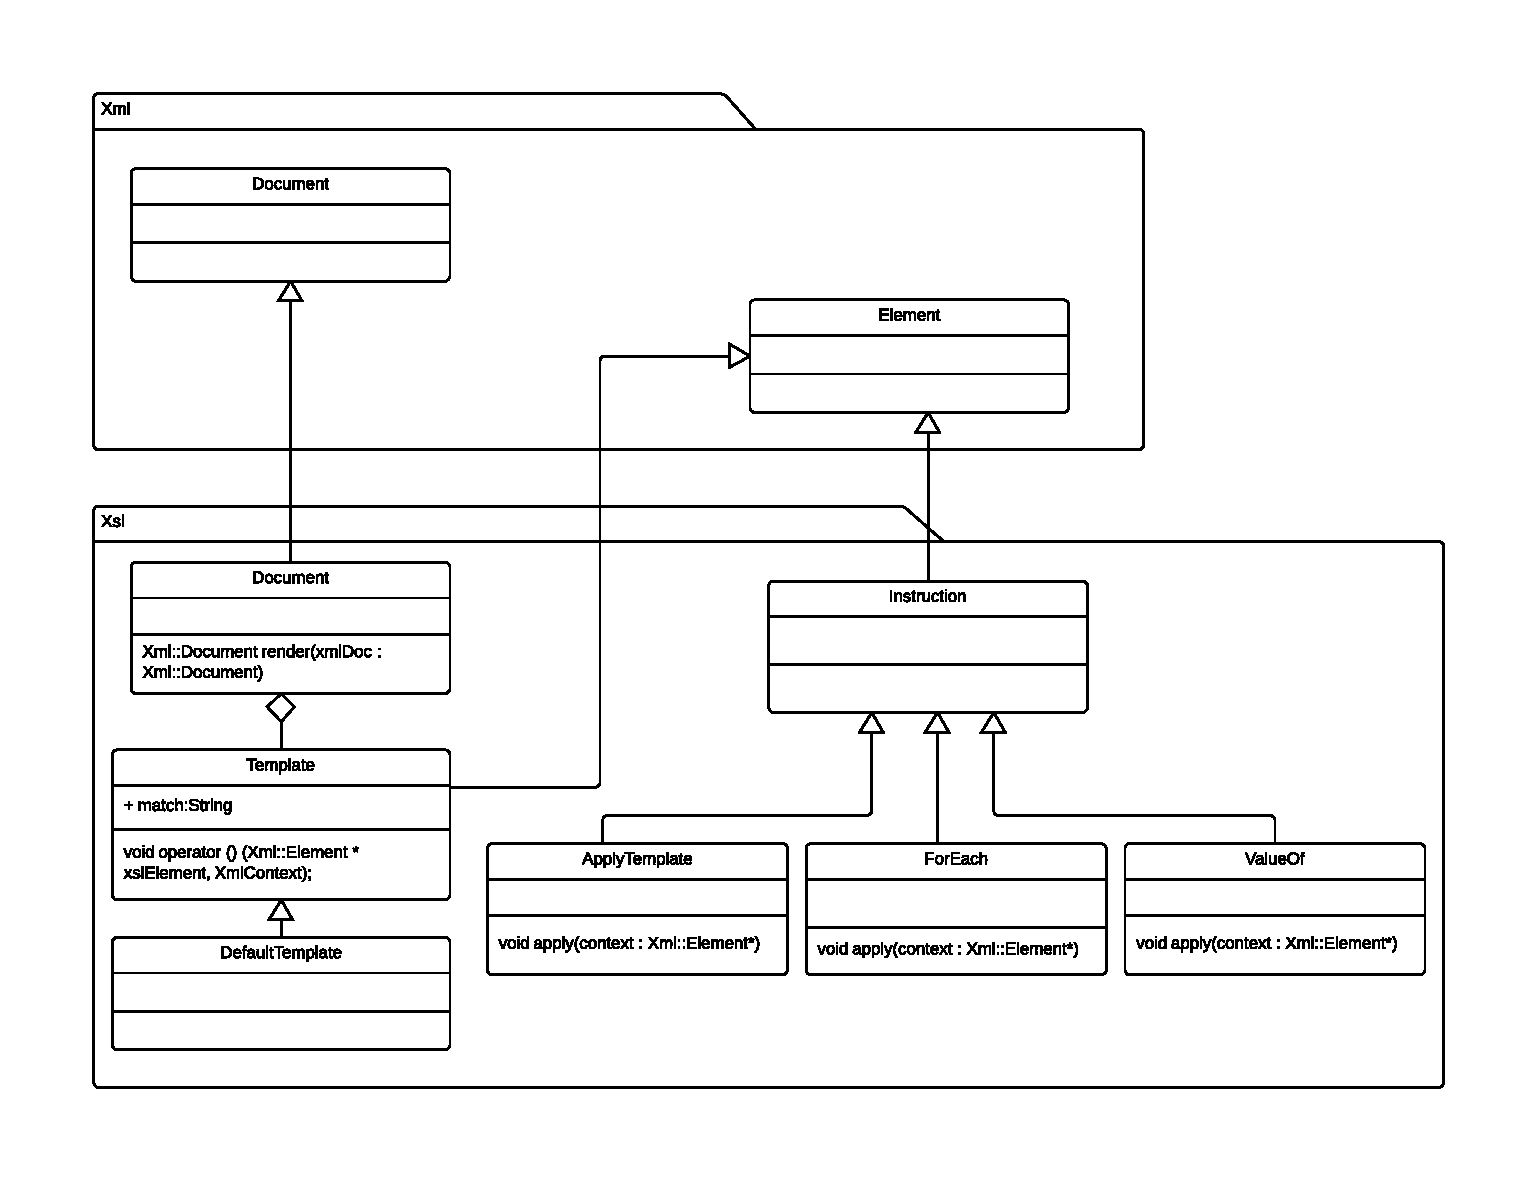
\includegraphics[width=\linewidth]{images/xsl-uml-old.pdf}
    \caption{Ancienne conception du module XSL}
    \label{oldXslClassDiagram}
\end{figure}

Néanmoins, cette conception présente de nombreux inconvénients : En plus d'ajouter de nombreuses classe sans vraie valeur ajoutée, elle
nous forçait à reconstruire l'arbre \textit{XML} afin de convertir les tags XSL en objets dédiés. On ne profitait pas réellement d'un quelconque
polymorphisme non plus puisque cela demandait de toucher aux classes XML, alors que celles ci n'ont pas comme responsabilité de gérer toutes
les applications possibles de ce langage de représentation de données. Il aurait aussi fallu tester le namespace des éléments \textit{XML} parcourus
avant de les caster à la bonne classe, donc pas grand d’intérêt au "polymorphisme".

Nous avons donc choisis de passer à une architecture plus simple : pas d'héritage, enfin si. Mais d'aucune classe du \lstinline$namespace Xml$.
Simplement une map constante faisant officie de virtual table, la liaison entre le nom des instructions \textit{Xsl} et des foncteurs qui
génèrent des nœuds \textit{XML} à partir d'un contexte donné.

\begin{landscape}
\begin{figure}[h!]
    \centering
    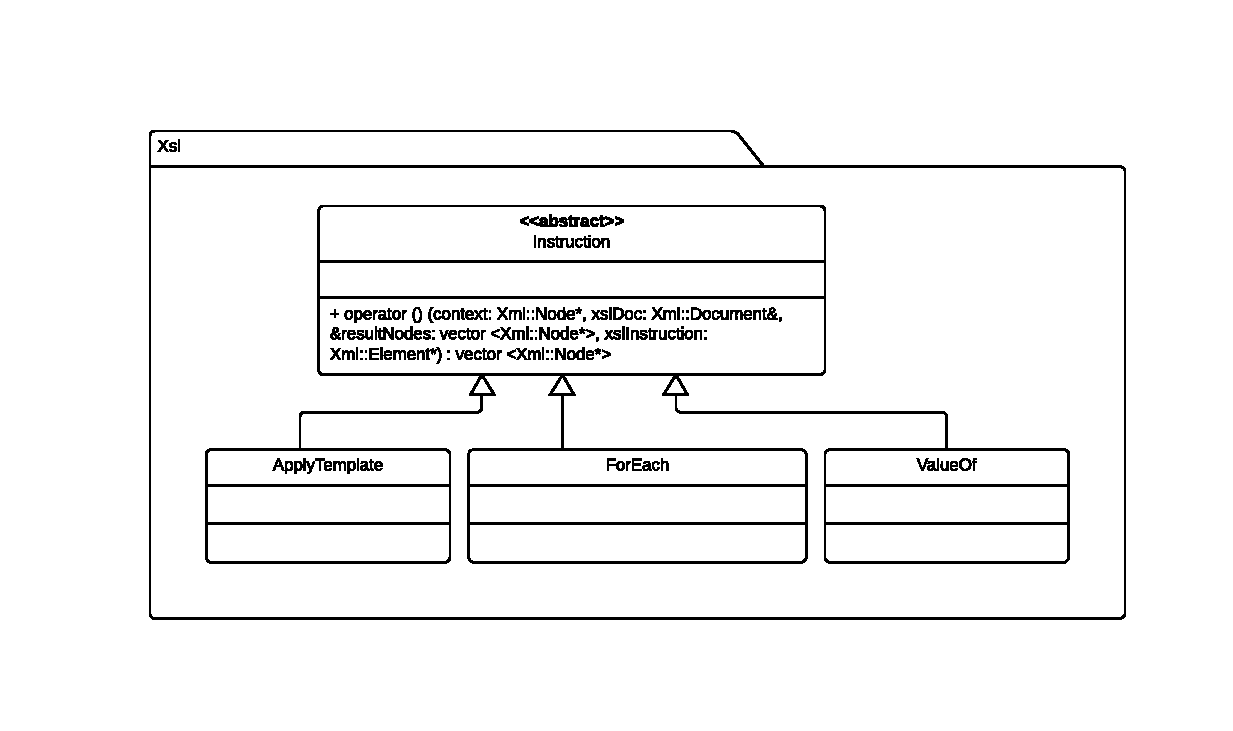
\includegraphics[width=\linewidth]{images/xsl-uml.pdf}
    \caption{Diagramme de classe des instructions XSL}
    \label{xslClassDiagram}
\end{figure}
\end{landscape}


\section{Vue globale de l'algorithme}

L'algorithme de transformation \textit{XSL} s’exécute de manière récursive et bascule continuellement entre le document \textit{XSL} et le
document \textit{XML} à transformer.

Un même algorithme s'exécute pour chaque nœud (à quelques exceptions citées ci-dessous) :

\begin{enumerate}
    \item Si le nœud n'est pas un élément, on le rajoute directement au résultat.
    \item Si un \textit{template} correspond à ce nœud, on l'applique (plus sur l'application des templates ci-dessous) en prenant ce nœud comme \textit{contexte} et on ajoute le résultat de cette application au nœud en cours de génération.
    \item Sinon, on ré-applique le même algorithme sur tous ses enfants, en ayant comme contexte l'élément actuel et en concaténant les résultats des applications de l'algorithme à tous le fils.
\end{enumerate}

La transformation \textit{XSL} débute en appliquant cet algorithme à la racine du document \textit{XML} à transformer, et se propage par récursions successives
à la totalité du document.

\section{Templates}

Les \textit{templates} sont les seuls fils de la racine (\textit{stylesheet}) d'un document \textit{XSL} et se présentent de la manière suivante :

\begin{lstlisting}[frame=single]
    <xsl:template match="cd/title">
        <tagxml></tagxml>
        <xsl:uneinstruction select="untag/unautretag"/>
    </xsl:template>
\end{lstlisting}

Ils peuvent contenir des tags \textit{XML} "normaux", ainsi que des instructions XSL.
On dit qu'un template \textit{match} un élément si l'élément est compatible avec la valeur de l'attribut \textit{match} du template, par exemple :

Si un élément XML a comme nom "unautretag" et est le fils d'un élément qui a comme nom "untag", il match le template vu ci-dessus.

Si un élément \textit{match} deux templates différents, on choisira celui qui est le plus spécifique.
Par exemple~: s'il y a deux templates \textit{"catalog/cd"} et \textit{"cd"}, c'est le premier qui sera appliqué pour les éléments "cd" fils de "catalog".

Quand on applique un template, on va renvoyer une liste de nœuds résultants (qui vont en général être ajoutés comme fils d'un document ou d'un élément). Cette liste est générée de la manière suivante :\\

\begin{enumerate}
    \item Les nœuds qui ne sont pas des éléments \textit{XML} sont rajoutés directement.
    \item Les nœuds qui sont des éléments \textit{XML}, mais pas \textit{XSL}, sont clonés. On applique alors  puis considérés comme des templates (car pouvant contenir des instructions \textit{XSL}) et appliqués avec comme contexte le nœud d'application de la transformation \textit{XSL}.
    \item Les éléments \textit{XSL} sont appliqués avec comme contexte le nœud d'application de la transformation \textit{XSL}. Tous les nœuds résultants de cette application sont ajoutés à la liste des nœuds générés par l'application du template.
\end{enumerate}

\section{Instructions XSL}

    \subsection{apply-template}
        Apply-template consiste à appliquer un template au noeud correspondant au chemin indiqué par l'expression XPath de l'attribut "select". Ce template doit se trouver dans la feuille de style Xsl que l'on est en train de parcourir pour transformer le document Xml. Si l'attribut select vaut "X" et qu'il existe dans le Xml le noeud correspondant au chemin de X dans le contexte courant, il doit donc exister dans le Xsl :
        \begin{lstlisting}[frame=single]
            <xsl:template match="X">
                ...........
                ...........
            </xsl:template>
        \end{lstlisting}.
         L'idée est alors de réappliquer le template trouvé à l'élément correspondant à X depuis le contexte courant de lecture du xml.
         Le template est appliqué et relance le traitement du Xml par l'appel des fonctions d'application de template habituelles.
         L'attribut "select" est optionnel, dans le cas de son absence, il faut alors chercher et appliquer les templates correspondants à tous les Noeuds Xml du contexte Xml courant, non récursivement. C'est à dire que si ces enfants ont des enfants, apply-templates ne forcera pas l'application des templates leurs correspondants

    \subsection{value-of}
        Value-of est une instruction Xsl permettant de retourner la valeur textuelle des éléments contenus au chemin indiqué par l'expression XPath requise comme paramêtre de "select". Cette instruction procède par récursion, c'est à dire que même les éléments textuels des éléments enfants sont affichés. Tout les textes retournés sont concatainés à l'emplacement de l'instruction Value-of.
        Value-of permet également d'afficher la valeur d'un attribut d'un noeud. En effet, en précisant @nomdelattribut en bout de chemin de l'expression XPath, la valeur de l'attribut appartenant à l'élément correspondant à l'expression XPath sera affichée.

    \subsection{for-each}
        For-each permet d'appliquer le templates contenus dans l'élément "for-each" à tous les noeuds dont le chemin est celui de l'expression XPath indiqué dans l'attribut "select" de for-each. Pour cela, il faut récupérer dans le document Xml tous les noeuds correspondants au XPath, puis appliquer à chacun le template contenu entre les balises for-each, comme ci c'était un template normal dans le déroulement de nos algorithmes. On retourne ensuite tout cela pour que ce soit ajouté à notre document transformé.

\section{Limites}

Bien qu'elle couvre les instructions XSL les plus courantes, avec un support extensif de nombreux cas spéciaux,
notre implémentation reste relativement limitée pour les raisons suivantes~:

\begin{enumerate}
    \item Spécifications assez massives et parfois ambiguës (sur le concept)
    \item Grand nombre de cas particuliers / cas limites
    \item Quelques incohérences (comme le pseudo-XPath utilisé pour l'attribut match)
    \item Transformations complexes
\end{enumerate}

Parmi ces limitations~:

\begin{enumerate}
    \item Pas de support pour des instructions XSL assez utiles, comme xsl:copy-of
    \item Algorithme faillible à des boucles infinies causées par des appels infinis d'apply-template
    \item Mauvais support des opérations de sélection depuis la racine (parce que le pseudo-XPATH utilisé en XSL considère "/" comme le document XML, et non sa racine)
\end{enumerate}


	%\renewcommand{\chaptermark}[1]{\markboth{\MakeUppercase{#1}}{}}
	%\renewcommand{\sectionmark}[1]{\markright{#1}}

	%\addcontentsline{toc}{part}{Annexes}
	%\part*{Annexes}
	%\appendix
	%\include{implementationExercices}


    % ------------------------------------------------------------------- FOOTER
\end{document}
